\chapter{Results and Discussion}

\section{Introduction}

This chapter presents and discusses the results of the lyric reconstruction experiments. The previous chapter described the implementation of the experimental pipeline, including dataset preparation, prompt construction, lyric generation, evaluation, and the auxiliary mood preservation analysis. This chapter uses the outputs from those experiments to compare the performance of the final prompt variants.

The evaluation is based on eight final prompt variants applied to the same fixed sample of 50 English-language songs. Since each prompt variant generated one reconstructed lyric for each song, the final experiment set contains 400 reconstructed lyrics in total. Using the same song sample across all runs allows the results to be compared directly, since differences between runs are primarily due to the prompt design and vocabulary configuration rather than changes in the underlying dataset.

The analysis is organised around the main evaluation dimensions introduced in Chapter 4. These include structural control, lexical adherence, reference similarity, semantic similarity, diversity, repetition, and auxiliary mood preservation. The aim is not to identify a single metric as the definitive measure of reconstruction quality. Instead, the chapter considers how different prompt variants perform across multiple dimensions, since lyric reconstruction requires a balance between preserving source-song information and producing coherent lyric-like text.

The chapter first gives an overview of the final experiment outputs, then analyses the results by evaluation category. It then discusses the auxiliary mood preservation experiments, including the limitations of classifier-based mood prediction and the use of lyric-derived affect analysis. Finally, the chapter compares the prompt variants overall and summarises the main findings, limitations, and implications for prompt-based lyric reconstruction. The emphasis is therefore on comparative interpretation: identifying which prompt strategies improve particular aspects of reconstruction, and where trade-offs occur between competing evaluation objectives.


\section{Overview of Final Experiment Outputs}

All final reconstruction experiments completed successfully. Each final prompt variant was applied to the same fixed sample of 50 English-language songs, producing one reconstructed lyric per song. Across the eight final prompt variants, this resulted in 400 reconstructed lyrics. Each run produced the expected output files, including the rendered prompt dataset, generated lyrics, per-song evaluation file, and summary evaluation file.

Table~\ref{tab:main_results_overview} provides an overview of the main run-level results. The table reports a selected set of metrics that represent the main evaluation dimensions used in this dissertation: structural control, lexical adherence, reference similarity, semantic similarity, and repetition. The detailed discussion of each metric group is provided in the following sections.

\begin{table}[H]
\centering
\renewcommand{\arraystretch}{1.2}
\caption{Overview of selected evaluation results for the final prompt variants. Higher values indicate better performance except for repetition, where lower values indicate fewer repeated lines.}
\label{tab:main_results_overview}
\begin{tabular}{
>{\raggedright\arraybackslash}p{0.24\textwidth}
>{\centering\arraybackslash}p{0.11\textwidth}
>{\centering\arraybackslash}p{0.11\textwidth}
>{\centering\arraybackslash}p{0.11\textwidth}
>{\centering\arraybackslash}p{0.11\textwidth}
>{\centering\arraybackslash}p{0.10\textwidth}
>{\centering\arraybackslash}p{0.11\textwidth}
}
\hline
Variant & Structure & Keyword & Weighted & Jaccard & BERT F1 & Repetition \\
\hline
Baseline LyCon-style & 1.52 & 0.765 & 0.760 & 0.352 & 0.810 & 0.140 \\
Structured & 4.00 & 0.733 & 0.750 & 0.326 & 0.806 & 0.442 \\
Frequency-aware & 4.00 & 0.775 & 0.800 & 0.355 & 0.807 & 0.444 \\
Raw vocabulary & 1.88 & 0.777 & 0.803 & 0.333 & 0.809 & 0.208 \\
Top-20 vocabulary & 2.30 & 0.823 & 0.825 & 0.236 & 0.801 & 0.264 \\
Top-100 vocabulary & 1.66 & 0.758 & 0.760 & 0.407 & 0.811 & 0.168 \\
Minimal control & 2.84 & 0.606 & 0.623 & 0.276 & 0.802 & 0.268 \\
Strong control & 4.00 & 0.824 & 0.846 & 0.367 & 0.807 & 0.426 \\
\hline
\end{tabular}
\renewcommand{\arraystretch}{1.0}
\end{table}

The metrics in Table~\ref{tab:main_results_overview} should be interpreted according to their evaluation role. Higher structure, keyword, weighted, Jaccard, and BERTScore values indicate stronger performance, while a lower repetition value indicates fewer repeated lines. The table therefore provides an overview of the main trade-offs rather than a single ranking of prompt variants.

The overview shows that no single prompt variant is best on every metric. Instead, the results reveal trade-offs between different forms of reconstruction quality. Strong control performs strongly on structure and lexical adherence, while the Top-100 vocabulary variant achieves the highest reference similarity and semantic similarity scores. By contrast, minimal control produces weaker lexical adherence, suggesting that looser prompts give the model more freedom but reduce reconstruction fidelity. These patterns are examined in more detail in the following sections.


\section{Structural Control Results}

The first evaluation dimension concerns the structural organisation of the generated lyrics. This is important because lyric reconstruction is not only a matter of recovering relevant words from the source song, but also of arranging the output into a recognisable lyrical form. Several prompt variants explicitly instructed the model to produce sections such as Verse 1, Chorus, Verse 2, and Chorus, while other variants left the structure more open.

The clearest result is that explicit structural prompting was highly effective. The Structured, Frequency-aware, and Strong control variants all achieved an average structure score of 4.00 and an average structure order match of 1.00. This means that, across the 50 generated lyrics in each of these runs, the required section labels were consistently present and appeared in the expected order. These results show that the language model followed direct structural instructions reliably when they were included in the prompt.

\begin{figure}[H]
\centering
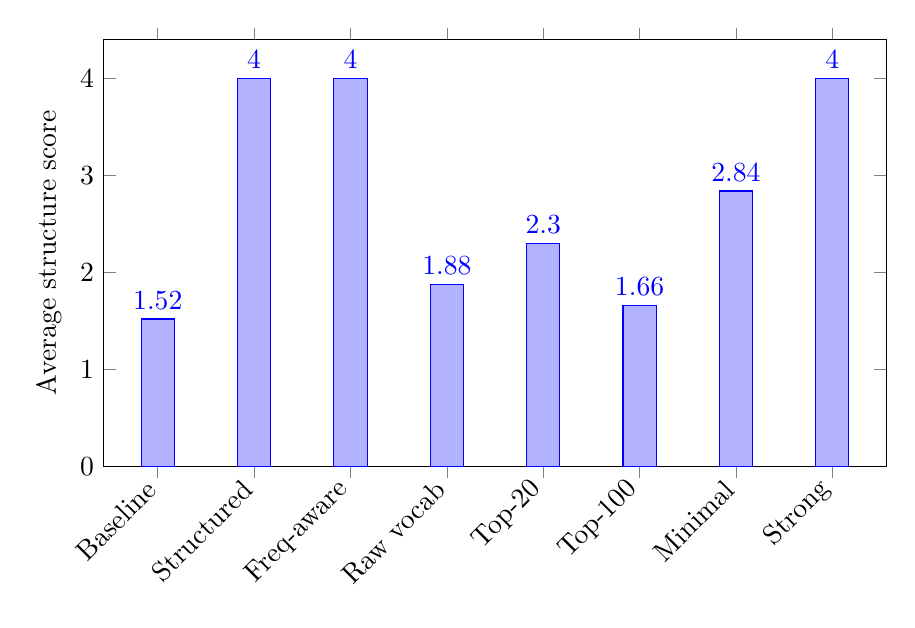
\begin{tikzpicture}
\begin{axis}[
    ybar,
    width=0.95\textwidth,
    height=7cm,
    ymin=0,
    ymax=4.4,
    ylabel={Average structure score},
    symbolic x coords={
        Baseline,
        Structured,
        Freq-aware,
        Raw vocab,
        Top-20,
        Top-100,
        Minimal,
        Strong
    },
    xtick=data,
    x tick label style={rotate=45, anchor=east},
    nodes near coords,
    nodes near coords align={vertical},
    bar width=12pt,
    enlarge x limits=0.08,
]
\addplot coordinates {
    (Baseline,1.52)
    (Structured,4.00)
    (Freq-aware,4.00)
    (Raw vocab,1.88)
    (Top-20,2.30)
    (Top-100,1.66)
    (Minimal,2.84)
    (Strong,4.00)
};
\end{axis}
\end{tikzpicture}
\caption{Average structure score across the final prompt variants. Variants with explicit structural instructions achieved the maximum score.}
\label{fig:structure_score_by_variant}
\end{figure}

By comparison, the Baseline LyCon-style variant achieved a lower average structure score of 1.52 and an average structure order match of 0.38. This indicates that, without explicit structural requirements, the model sometimes generated section-like lyrics but did not consistently follow the target structure. The Raw vocabulary and Top-100 vocabulary variants also had relatively low structure scores, at 1.88 and 1.66 respectively. These variants were designed primarily to test vocabulary representation and vocabulary size rather than structure, so this outcome is expected.

The Minimal control variant achieved a structure score of 2.84 and an order match of 0.70. This is higher than the baseline, even though the prompt was less constrained overall. One possible explanation is that the model has learned common lyric conventions from pretraining and can produce verse-chorus-like formatting even when not strongly instructed. However, the result is still below the explicitly structured variants, suggesting that implicit lyric knowledge is less reliable than direct structural guidance.

These findings support the value of structural prompt control. When the prompt explicitly specified the expected lyric organisation, the model produced outputs that matched the required structure consistently. This is one of the strongest findings in the experiment, because the difference between structured and non-structured conditions is clear across the structure metrics. This suggests that formal lyric structure is one of the more controllable aspects of the reconstruction task, because it can be specified directly in the prompt rather than inferred from the bag-of-words representation. However, the later repetition analysis shows that stronger structural control may also encourage repeated lines or formulaic chorus behaviour, so structural success needs to be considered alongside diversity and repetition.


\section{Lexical Adherence Results}

The second evaluation dimension concerns lexical adherence: the extent to which the generated lyrics use the vocabulary supplied in the prompt. This is central to the dissertation because the reconstruction task is based on generating lyrics from a reduced bag-of-words representation. If a prompt variant produces fluent lyrics but does not use the supplied vocabulary, then it is less successful as a reconstruction method.

The strongest lexical adherence was achieved by the Strong control and Top-20 vocabulary variants. Strong control achieved the highest overall keyword coverage, with an average keyword coverage of 0.824. It also achieved the highest weighted keyword coverage, at 0.846, and the highest top keyword coverage, at 0.896. This suggests that the strong prompt instructions were effective at encouraging the model to use the supplied vocabulary, especially the most important vocabulary terms.

The Top-20 vocabulary variant achieved a very similar average keyword coverage of 0.823 and a weighted keyword coverage of 0.825. However, this result should be interpreted carefully. Because the Top-20 condition provides a smaller vocabulary list, it is easier for the model to cover a larger proportion of the supplied words. Its high keyword coverage therefore indicates strong use of the compact vocabulary signal, but it does not necessarily mean that it reconstructs more of the original lyric overall. This becomes clearer in the reference similarity results, where the Top-20 condition performs less strongly.

The Frequency-aware and Raw vocabulary variants also performed well on lexical adherence. Frequency-aware achieved a keyword coverage of 0.775 and a weighted keyword coverage of 0.800, while Raw vocabulary achieved a keyword coverage of 0.777 and a weighted keyword coverage of 0.803. These results suggest that both frequency information and broader surface-level vocabulary can help the model incorporate supplied lexical cues. The Raw vocabulary condition also produced the highest keyword density, at 0.496, meaning that a larger proportion of its generated words came from the supplied vocabulary list. However, high keyword density does not automatically indicate better reconstruction quality, since it may also reflect heavier reuse of common or less informative tokens.

By contrast, the Minimal control variant showed the weakest lexical adherence. It achieved an average keyword coverage of 0.606 and a weighted keyword coverage of 0.623, both of which were the lowest among the final prompt variants. This supports the expectation that looser prompting gives the model more freedom but reduces its tendency to use the supplied bag-of-words representation. In other words, minimal control may allow the model to produce plausible lyrics, but it weakens the reconstruction link between the generated output and the source song representation.

Overall, the lexical adherence results show that prompt wording has a clear effect on vocabulary use. Stronger instructions lead to greater use of supplied lexical cues, while reduced constraints lead to lower keyword coverage. This supports the central assumption of the dissertation: when reconstructing from bag-of-words constraints, the model needs explicit guidance to treat the vocabulary as reconstruction evidence rather than optional inspiration. However, lexical adherence must be interpreted alongside other metrics. A prompt can achieve high keyword coverage by using a smaller vocabulary list or by repeating supplied terms more often, so keyword coverage alone is not sufficient to determine the best reconstruction method. The following sections therefore compare these lexical findings with reference similarity, semantic similarity, diversity, and repetition.


\section{Reference and Semantic Similarity Results}

The third evaluation dimension concerns similarity between the generated lyrics and the original reference lyrics. This is important because the task is framed as lyric reconstruction rather than unconstrained lyric generation. While lexical adherence measures whether the generated output uses the supplied vocabulary, reference similarity evaluates whether the output also overlaps with the original lyrics more broadly.

The strongest reference similarity was achieved by the Top-100 vocabulary variant. This variant obtained the highest reference Jaccard similarity, at 0.407, as well as the highest BERTScore F1, at 0.811. It also achieved the highest reference unigram recall, at 0.639. These results suggest that providing a larger vocabulary list gives the model access to more of the source song's lexical material, increasing the chance that the generated output overlaps with the reference lyric. This is consistent with the role of bag-of-words representations as partial evidence of the source text: increasing the vocabulary budget exposes more source-song information, which improves overlap-based and semantic similarity measures.

By contrast, the Top-20 vocabulary variant achieved the lowest reference Jaccard similarity, at 0.236, and the lowest BERTScore F1, at 0.801. This is an important contrast with the lexical adherence results. Although Top-20 achieved high keyword coverage, it did so using a much smaller vocabulary list. The model could cover many of the supplied words, but the reduced lexical budget limited how much of the original reference lyric could be represented. This shows that high keyword coverage does not necessarily imply high reconstruction similarity.

The Strong control variant performed well, but it was not the strongest condition for reference similarity. It achieved a reference Jaccard similarity of 0.367 and a BERTScore F1 of 0.807. These scores are below the Top-100 variant but above most other controlled variants. This suggests that strong prompting improves the model's adherence to the supplied reconstruction cues, but the top-50 vocabulary budget still limits the amount of reference material available to the model compared with the Top-100 condition.

The Baseline LyCon-style and Frequency-aware variants produced similar reference similarity results. The baseline achieved a reference Jaccard similarity of 0.352 and a BERTScore F1 of 0.810, while the Frequency-aware variant achieved a reference Jaccard similarity of 0.355 and a BERTScore F1 of 0.807. The similarity between these results suggests that adding structure and frequency information did not necessarily improve reference overlap by itself. Instead, these controls appear to affect other dimensions more strongly, such as structure and lexical prioritisation.

Overall, the reference and semantic similarity results reveal a different pattern from the structural and lexical results. Strong control is the best overall condition for controlled reconstruction, but the Top-100 vocabulary variant is the strongest when the goal is maximising similarity to the reference lyrics. This highlights an important trade-off in lyric reconstruction: increasing the amount of lexical information can improve reference similarity, while stronger prompt constraints can improve structural and lexical control. The best prompt design therefore depends on whether the priority is reference overlap, formal structure, or balanced reconstruction performance.

\section{Diversity and Repetition Results}

The fourth evaluation dimension concerns diversity and repetition in the generated lyrics. This is important because a reconstruction method should not only recover vocabulary from the source song, but also produce varied and coherent lyric-like text. In lyric generation, some repetition is expected because choruses, hooks, and refrains are common features of songs. However, excessive repetition can indicate that the model is relying too heavily on repeated lines or phrases rather than producing varied lyrical content.

The results show a clear trade-off between structural control and repetition. The variants with explicit structural requirements tended to produce higher repeated line ratios. The Structured variant had a repeated line ratio of 0.442, the Frequency-aware variant had a repeated line ratio of 0.444, and the Strong control variant had a repeated line ratio of 0.426. These are among the highest values across the final experiments. This suggests that when the model is instructed to follow a verse-chorus structure, it often repeats chorus-like material or reuses lines more heavily.

By contrast, the Baseline LyCon-style and Top-100 vocabulary variants produced lower repeated line ratios. The baseline had a repeated line ratio of 0.140, while the Top-100 variant had a repeated line ratio of 0.168. These variants did not enforce the same strict structural organisation, which may have allowed the model to generate more varied line sequences. This supports the interpretation that explicit structure improves formal organisation, but may also encourage more formulaic repetition.

The diversity metrics also show that the Top-100 vocabulary variant produced the highest lexical diversity. It achieved the highest distinct-1 score, at 0.620, and one of the highest distinct-2 scores, at 0.846. This is consistent with the fact that the Top-100 prompt provides a larger vocabulary budget, giving the model access to a wider set of lexical cues. The Baseline LyCon-style variant also performed strongly on distinct-2, at 0.863, suggesting that less constrained prompting can support varied phrasing.

The Minimal control variant produced the longest outputs on average, with an average word count of 245.70 and an average line count of 36.12. However, this did not translate into stronger reconstruction performance. As shown in the lexical adherence results, Minimal control had the weakest keyword coverage, suggesting that the additional length came with reduced adherence to the supplied vocabulary. This supports the idea that longer outputs are not necessarily better reconstructions.

Overall, the diversity and repetition results show that prompt control introduces a trade-off. Strong structural instructions help the model produce recognisable lyric sections, but they also increase the risk of repeated lines. This metric therefore needs to be interpreted in context: repetition is a normal feature of lyrics, but high repeated-line ratios may indicate that the model is satisfying structure by duplicating lines rather than developing new lyrical material. Larger or less constrained vocabulary conditions can produce more diverse outputs, but may provide weaker formal control. These findings suggest that lyric reconstruction requires balancing structure, lexical adherence, and diversity rather than maximising any single metric in isolation.


\section{Mood Preservation Analysis}

The final evaluation dimension concerns mood preservation. Since mood information was included in the prompt through the valence-arousal mapping, it was useful to investigate whether the reconstructed lyrics preserved affective characteristics of the source songs. This analysis was treated as auxiliary rather than as the primary evaluation, because mood preservation is difficult to measure automatically and the available affective labels are not direct human annotations of lyric emotion.

Two types of mood preservation analysis were carried out. The first used classifier-based mood prediction, where models were trained to predict mood-related labels from lyrics. The second used lyric-derived affect analysis based on word-level valence and arousal ratings. The classifier-based approach tested whether generated lyrics could be assigned the same mood category as the original song, while the lyric-derived approach compared generated and reference lyrics directly in an affective word-rating space.

\begin{table}[H]
\centering
\renewcommand{\arraystretch}{1.2}
\caption{Summary of mood preservation analysis methods and main outcomes.}
\label{tab:mood_preservation_summary}
\begin{tabular}{
>{\raggedright\arraybackslash}p{0.26\textwidth}
>{\raggedright\arraybackslash}p{0.28\textwidth}
>{\raggedright\arraybackslash}p{0.34\textwidth}
}
\hline
Method & Main outcome & Interpretation \\
\hline
12-mood classifier & Best macro F1: 0.185 & Too unreliable for fine-grained mood preservation evaluation. \\
4-mood quadrant classifier & Macro F1: 0.422 & More stable than 12-mood prediction, but still limited. \\
Binary valence/arousal classifiers & Valence macro F1: 0.656; arousal macro F1: 0.634 & Useful only as exploratory broad affect prediction. \\
Warriner lyric-derived affect & Strong control achieved lowest VA distance: 0.312 & Most useful auxiliary text-based mood preservation measure. \\
\hline
\end{tabular}
\renewcommand{\arraystretch}{1.0}
\end{table}

\subsection{Classifier-Based Mood Preservation}

The initial mood preservation approach used supervised lyric classifiers trained on Music4All songs that were not part of the 50-song reconstruction sample. The first formulation used the same 12 mood labels as the prompt construction process. This formulation exposed an important methodological limitation. The best 12-mood classifier achieved an average accuracy of 0.236 and a macro F1 score of 0.185 across repeated train-test splits. This indicates that fine-grained 12-way mood prediction from lyrics alone was not reliable enough to serve as a strong evaluation method.

Several reasons explain this limitation. First, the 12 mood labels are derived from angular sectors in the valence-arousal space, meaning that neighbouring moods can be close to each other. A song near a sector boundary may receive a different label from another song with very similar affective characteristics. Second, the dataset is imbalanced, with some moods appearing much more frequently than others. Third, and most importantly, the Music4All valence and energy values are song-level metadata rather than lyric-specific emotion annotations. These values may reflect audio properties such as tempo, instrumentation, rhythm, and production, while the classifier only receives lyric text.

To investigate whether the classifier limitation could be reduced, several alternative formulations were tested. These included linear classifiers with TF-IDF features, a hierarchical 12-mood classifier, a DistilBERT pilot, balanced 4-mood training, clean-margin filtering, separate binary valence and arousal classifiers, and valence-arousal regression. These attempts improved some aspects of performance, but did not remove the underlying problem. In particular, balancing the 4-mood training data did not improve the macro-level result, and the regression experiment still showed only moderate correlation with the original valence and arousal values. This suggests that the main difficulty is not only model choice or class imbalance, but the mismatch between song-level affect metadata and lyric-only input.

To reduce the difficulty of the task, broader classifier formulations were also tested. A 4-mood quadrant classifier achieved an average accuracy of 0.524 and a macro F1 score of 0.422. Binary valence and arousal classifiers performed better when the two affective dimensions were predicted separately, with average macro F1 scores of 0.656 for valence and 0.634 for arousal. These results suggest that broad affective direction is more predictable from lyrics than fine-grained mood labels, but the performance is still not strong enough to treat classifier-based mood preservation as definitive.

The binary valence and arousal classifiers were then applied to the generated lyrics to estimate whether the reconstructed lyrics preserved the original song's broad affective direction. Table~\ref{tab:binary_va_generated_mood_preservation} shows the proportion of generated lyrics that matched the original song's binary valence label, binary arousal label, and both labels together.

\begin{table}[H]
\centering
\renewcommand{\arraystretch}{1.2}
\caption{Classifier-based valence and arousal preservation on generated lyrics. Values show the proportion of generated lyrics matching the original song's binary valence and arousal labels.}
\label{tab:binary_va_generated_mood_preservation}
\begin{tabular}{
>{\raggedright\arraybackslash}p{0.36\textwidth}
>{\centering\arraybackslash}p{0.16\textwidth}
>{\centering\arraybackslash}p{0.16\textwidth}
>{\centering\arraybackslash}p{0.16\textwidth}
}
\hline
Prompt variant & Valence & Arousal & Both \\
\hline
Baseline LyCon-style & 0.70 & 0.80 & 0.56 \\
Frequency-aware & 0.66 & 0.76 & 0.50 \\
Minimal control & 0.60 & 0.80 & 0.50 \\
Top-20 vocabulary & 0.62 & 0.78 & 0.48 \\
Raw vocabulary & 0.62 & 0.80 & 0.46 \\
Strong control & 0.64 & 0.78 & 0.44 \\
Structured & 0.58 & 0.78 & 0.42 \\
Top-100 vocabulary & 0.56 & 0.70 & 0.36 \\
\hline
\end{tabular}
\renewcommand{\arraystretch}{1.0}
\end{table}

The classifier-based results suggest that the Baseline LyCon-style variant achieved the highest combined binary valence-arousal match rate, at 0.56. However, this result should be interpreted cautiously because it depends on classifiers with only moderate reliability. The classifier-based results are therefore useful mainly as exploratory evidence. They show that mood preservation can be investigated computationally, but they also reveal the difficulty of using song-level affect metadata as ground truth for lyric-only mood prediction.

\subsection{Lyric-Derived Affect Analysis}

Because of the limitations of classifier-based mood prediction, a second auxiliary analysis was carried out using lyric-derived affect scores. This method used word-level valence and arousal ratings from the Warriner lexicon to estimate the affective profile of both the reference lyrics and the generated lyrics. For each lyric, the analysis computed average valence and arousal over the words covered by the lexicon, then measured the distance between the generated lyric and the original reference lyric in this affective space.

This analysis provides a more directly text-based view of mood preservation. Unlike the classifier approach, it does not attempt to predict song-level valence or arousal metadata. Instead, it compares the affective vocabulary of the generated lyric with the affective vocabulary of the reference lyric. This makes the method better aligned with the text-only nature of the generated outputs, although it remains approximate because word-level ratings cannot capture full lyrical meaning, context, irony, or musical delivery.

Table~\ref{tab:warriner_generated_mood_preservation} shows the lyric-derived affect preservation results for the generated runs. Lower values indicate that the generated lyrics are closer to the reference lyrics in Warriner valence-arousal space.

\begin{table}[H]
\centering
\renewcommand{\arraystretch}{1.2}
\caption{Lyric-derived affect preservation across generated runs using Warriner valence-arousal distance. Lower values indicate closer affective similarity to the reference lyrics.}
\label{tab:warriner_generated_mood_preservation}
\begin{tabular}{
>{\raggedright\arraybackslash}p{0.42\textwidth}
>{\centering\arraybackslash}p{0.30\textwidth}
}
\hline
Prompt variant & Average VA distance \\
\hline
Strong control & 0.312 \\
Top-100 vocabulary & 0.347 \\
Baseline LyCon-style & 0.367 \\
Frequency-aware & 0.380 \\
Raw vocabulary & 0.387 \\
Top-20 vocabulary & 0.399 \\
Structured & 0.415 \\
Minimal control & 0.452 \\
\hline
\end{tabular}
\renewcommand{\arraystretch}{1.0}
\end{table}

The lyric-derived affect results were more consistent with the main reconstruction findings. The Strong control variant achieved the lowest average valence-arousal distance, at 0.312, indicating the closest affective match to the reference lyrics under this measure. The Top-100 vocabulary variant was second, with an average distance of 0.347, followed by the Baseline LyCon-style variant at 0.367. The Minimal control variant had the largest average distance, at 0.452.

These results suggest that stronger prompt control can help preserve the affective word profile of the source lyrics. This is consistent with the earlier lexical adherence results, where Strong control showed the highest weighted keyword coverage. If the generated lyrics make stronger use of the supplied source vocabulary, they are also more likely to preserve affective lexical cues from the original lyrics. At the same time, the Warriner analysis should not be treated as a complete measure of mood preservation. It is best understood as an auxiliary text-based indicator that complements the main reconstruction metrics.

\section{Overall Comparison of Prompt Variants}

The results show that no single prompt variant is best on every metric. Instead, each variant reflects a different trade-off between structure, lexical adherence, reference similarity, diversity, and mood preservation. This means that the best prompt strategy depends on how reconstruction quality is defined.

Overall, the Strong control variant provides the best balance across the main evaluation dimensions. It achieved a perfect structure score of 4.00 and a structure order match of 1.00, showing that it consistently followed the required lyric organisation. It also achieved the highest keyword coverage, at 0.824, the highest weighted keyword coverage, at 0.846, and the highest top keyword coverage, at 0.896. In the lyric-derived affect analysis, it also produced the lowest average valence-arousal distance from the reference lyrics, at 0.312. These results suggest that combining structure, vocabulary, and frequency constraints gives the model the strongest overall reconstruction guidance.

However, Strong control was not the best variant for reference similarity. The Top-100 vocabulary variant achieved the highest reference Jaccard similarity, at 0.407, and the highest BERTScore F1, at 0.811. This indicates that providing a larger lexical budget helps the model recover more reference-related content. The Top-100 variant therefore performs best when the priority is similarity to the original lyrics, even though it does not provide the same level of structural control as Strong control.

The Minimal control variant provides the clearest contrast. It achieved the lowest keyword coverage, at 0.606, and the largest lyric-derived affect distance, at 0.452. Although it allowed the model greater freedom and produced longer outputs on average, it was less effective as a reconstruction method. This supports the conclusion that prompt control is important when generating from a reduced bag-of-words representation.

Table~\ref{tab:best_variants_by_dimension} summarises the best-performing variants by evaluation dimension.

\begin{table}[H]
\centering
\renewcommand{\arraystretch}{1.2}
\caption{Best-performing prompt variants by evaluation dimension.}
\label{tab:best_variants_by_dimension}
\begin{tabular}{
>{\raggedright\arraybackslash}p{0.30\textwidth}
>{\raggedright\arraybackslash}p{0.26\textwidth}
>{\raggedright\arraybackslash}p{0.32\textwidth}
}
\hline
Evaluation dimension & Best variant & Main reason \\
\hline
Structural control & Structured, Frequency-aware, Strong control & Perfect structure score and order match. \\
Lexical adherence & Strong control & Highest keyword and weighted keyword coverage. \\
Reference similarity & Top-100 vocabulary & Highest Jaccard similarity and BERTScore F1. \\
Lyric-derived affect preservation & Strong control & Lowest valence-arousal distance from reference lyrics. \\
Lowest repetition & Baseline LyCon-style & Lowest repeated line ratio among the final variants. \\
\hline
\end{tabular}
\renewcommand{\arraystretch}{1.0}
\end{table}

Taken together, these findings suggest that Strong control is the strongest overall configuration, while Top-100 vocabulary is the strongest configuration for reference similarity. The results therefore support the main idea of the dissertation: prompt-based lyric reconstruction benefits from controlled use of lexical, structural, and affective cues, but different forms of control improve different aspects of the output.

\section{Discussion of Key Findings}

The first key finding is that prompt design has a clear effect on lyric reconstruction behaviour. The same 50 songs and the same language model were used across all final experiments, so the differences between runs can be attributed mainly to the way information was presented in the prompt. This supports the decision to treat prompt design as the main experimental variable in the dissertation. This finding is also consistent with the broader literature on controlled text generation, where explicit constraints are often used to steer model output towards desired content or form.

The second key finding is that explicit structural instructions are highly effective. Prompt variants that required a Verse 1, Chorus, Verse 2, Chorus structure achieved perfect structure scores and order matches. This shows that the language model can reliably follow formal lyric-structure constraints when they are stated clearly. However, this benefit comes with a trade-off, since structured variants also showed higher repeated line ratios. This reflects a wider tension in controlled generation between controllability and diversity.

The third key finding is that lexical control improves reconstruction adherence. Strong control achieved the best lexical adherence results, while Minimal control performed worst. This indicates that when the model is given a reduced bag-of-words representation, it benefits from explicit instructions to use the supplied vocabulary. Without these instructions, the model may generate plausible lyrics but becomes less tied to the source song representation.

The fourth key finding is that reference similarity benefits from a larger vocabulary budget. The Top-100 vocabulary variant achieved the highest reference Jaccard similarity and BERTScore F1. This suggests that giving the model more source vocabulary increases the chance of recovering reference-related content. This finding follows the intuition behind lexical-constraint and bag-of-words approaches: a richer lexical representation provides more evidence about the source text. However, this does not automatically make it the best overall prompt, because Top-100 did not achieve the strongest structure or lexical-control results.

The fifth key finding concerns mood preservation. Classifier-based mood preservation was difficult because the available valence and arousal labels are song-level metadata rather than lyric-specific emotion annotations. This is consistent with the broader challenge of lyric emotion analysis, where text-only models may not fully recover affective labels that are influenced by audio, performance, or production features. The lyric-derived Warriner analysis provided a more text-based auxiliary measure and suggested that Strong control best preserved the affective word profile of the reference lyrics. This finding supports the broader pattern that stronger prompt control helps preserve source-song characteristics.

Overall, the results show that lyric reconstruction from bag-of-words style inputs is possible, but it involves balancing competing objectives. More control improves structure and vocabulary use, while larger vocabulary improves reference similarity. Too little control weakens reconstruction adherence, but too much structure may increase repetition. The most successful approach is therefore not simply the most free or the most constrained prompt, but a prompt that balances structure, lexical guidance, and flexibility.

\section{Limitations}

Several limitations should be considered when interpreting the results. First, the final reconstruction experiments were conducted on a sample of 50 songs. Although the same songs were used across all prompt variants, which supports fair comparison, a larger sample would provide stronger evidence about how well the findings generalise across genres, artists, and lyric styles.

Second, the evaluation relies heavily on automatic metrics. These metrics are useful for comparing prompt variants consistently, but they cannot fully capture lyric quality, originality, coherence, emotional impact, or artistic value. For example, a generated lyric may achieve high keyword coverage while still sounding unnatural, or it may have low reference overlap while still being a coherent lyric. Human evaluation would therefore be needed to complement the automatic results.

Third, the reference lyrics are used both to extract the bag-of-words vocabulary and to evaluate reconstruction similarity. This is appropriate for the reconstruction setting, but it also means that the task is not equivalent to generating lyrics from metadata alone. The results should therefore be interpreted as reconstruction from reduced lyric-derived cues, not as fully independent lyric generation.

Fourth, the mood preservation analysis is limited by the available affective labels. Music4All valence and energy values are song-level metadata and may reflect audio features as well as lyric content. This makes lyric-only mood classification difficult. Although the Warriner analysis provides a more text-based alternative, it is still based on word-level ratings and cannot fully capture contextual meaning or musical delivery.

Fifth, the experiments use a single language model, \texttt{gpt-4o-mini}. Keeping the model fixed was useful for isolating the effect of prompt design, but the results may differ with other models or future versions of the same model. In addition, API-based generation can involve some variability, so the saved outputs and configuration snapshots are important for preserving the exact experimental record.

Sixth, the experiments evaluate one generated output per song and prompt variant. Sampling multiple outputs for each prompt would provide a better estimate of how stable each prompt strategy is, especially because language model outputs can vary across generations.

Finally, copyright constraints limit the extent to which original lyrics can be reproduced or qualitatively analysed in the dissertation. This makes the work more dependent on automatic metrics and short illustrative examples. Future work could address this through human evaluation protocols that do not require publishing long lyric excerpts.

\section{Chapter Summary}

This chapter presented and discussed the results of the final lyric reconstruction experiments. The experiments compared eight prompt variants across a fixed set of 50 songs, producing 400 reconstructed lyrics in total. The analysis showed that prompt design had a clear effect on reconstruction behaviour.

The Strong control variant provided the best overall balance across the main evaluation dimensions. It achieved perfect structural performance, the strongest lexical adherence, and the best lyric-derived affect preservation score. The Top-100 vocabulary variant achieved the strongest reference and semantic similarity, showing that a larger vocabulary budget helps recover more source-song content. The Minimal control variant performed weakest on lexical adherence, demonstrating that loose prompting reduces the connection between the generated lyric and the source representation.

The mood preservation experiments showed that classifier-based mood prediction is difficult when using song-level affect metadata as labels for lyric-only text. However, the lyric-derived affect analysis provided useful auxiliary evidence that stronger prompt control can better preserve the affective vocabulary profile of the original lyrics.

Overall, the results suggest that prompt-based lyric reconstruction benefits from combining lexical, structural, and affective cues. The strongest results were achieved when the prompt gave the model clear reconstruction guidance while still allowing enough flexibility to generate coherent lyrics. The next chapter concludes the dissertation by summarising the contributions, reflecting on the research questions, and outlining directions for future work.
